\documentclass[svgnames,11pt]{beamer}
\input{/home/tof/Documents/Cozy/latex-include/preambule_commun.tex}
\input{/home/tof/Documents/Cozy/latex-include/preambule_beamer.tex}
%\usepackage{pgfpages} \setbeameroption{show notes on second screen=left}
\author[]{Christophe Viroulaud}
\title{Programmation dynamique\\TP découpe d'une barre}
\date{\framebox{\textbf{Algo 26}}}
%\logo{}
\institute{Terminale - NSI}

\begin{document}
\begin{frame}
\titlepage
\end{frame}
\begin{frame}
    \frametitle{}

    Un ferrailleur découpe des barres métalliques pour la revente. Les barres, plus petites, obtenues sont utilisées dans diverses constructions (garde-corps, châssis, fenêtre\dots). Le prix de revente des barres n'est donc pas proportionnel à leur dimension.
\begin{center}
    \begin{tabular}{|*{9}{c|}}
        \hline
        Longueur & 1 & 2 & 3 & 4 & 5 & 6 & 8 & 10 \\
        \hline
        Prix & 2 & 5 & 8 & 10 & 11 & 14 & 17 & 20 \\
        \hline
    \end{tabular}
\end{center}

\end{frame}
\begin{frame}
    \frametitle{}

    \begin{framed}
        \centering Comment maximiser le prix de vente d'une barre?
    \end{framed}

\end{frame}
\section{Approche naïve}
\begin{frame}
    \frametitle{Approche naïve}

    Une formalisation mathématique du débitage d'une barre de longueur \texttt{\textbf{longueur}} permet d'écrire pour une première découpe de taille \texttt{\textbf{taille}}:
    $$prix\_max(longueur) = prix(taille) + prix\_max(longueur-taille)$$
    Si on effectue une première découpe \texttt{\textbf{taille}}, il reste une barre \texttt{\textbf{longueur-taille}}. L'objectif est de trouver le prix pour chaque découpe possible et ne garder que le prix maximum.

\end{frame}
\begin{frame}
    \frametitle{}

    \begin{activite}
        \begin{enumerate}
            \item Déterminer \emph{à la main} le prix maximal pour une barre de longueur 10.
            \item Construire \underline{le début} de l'arbre des possibilités de découpe permettant de calculer les prix de vente.
            \item Construire un dictionnaire associant la longueur de barre à son prix.
            \item Déterminer une fonction \textbf{récursive} permettant de calculer le prix maximal obtenu pour la découpe d'une barre. La fonction parcourra toutes les branches de l'arbre pour déterminer le prix maximum.  
        \end{enumerate}
        \end{activite}

\end{frame}
\begin{frame}
    \frametitle{Avant de regarder la correction}
\begin{center}
    \centering
    \includegraphics[width=3cm]{/home/tof/Documents/Cozy/latex-include/stop.png}
    \end{center}
{\Large
    \begin{itemize}
        \item Prendre le temps de réfléchir,
        \item Analyser les messages d'erreur,
        \item Demander au professeur.
    \end{itemize}
}
\end{frame}
\begin{frame}
    \frametitle{Correction}

    \begin{itemize}
        \item 3 découpes de taille 3: $8×3=24$
        \item 1 découpe de taille 1: $2×1=2$
    \end{itemize}
\begin{center}
    Le prix maximal obtenu est 26.
\end{center}
\end{frame}
\begin{frame}
    \frametitle{}
    \begin{center}
        \begin{tabular}{|*{9}{c|}}
            \hline
            Longueur & 1 & 2 & 3 & 4 & 5 & 6 & 8 & 10 \\
            \hline
            Prix & 2 & 5 & 8 & 10 & 11 & 14 & 17 & 20 \\
            \hline
        \end{tabular}
    \end{center}
    \begin{center}
        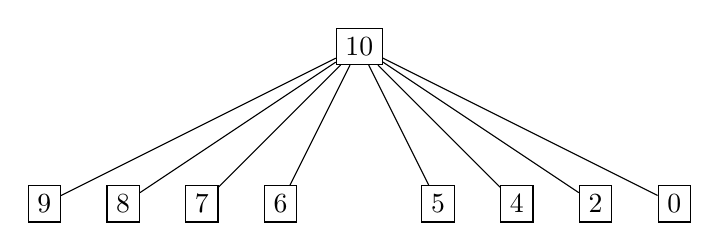
\begin{tikzpicture}
            \node[draw] (A) at (0,0) {10};
            \node[draw] (B) at (-4,-2) {9};
            \node[draw] (C) at (-3,-2) {8};
            \node[draw] (D) at (-2,-2) {7};
            \node[draw] (E) at (-1,-2) {6};
            \node[draw] (F) at (1,-2) {5};
            \node[draw] (G) at (2,-2) {4};
            \node[draw] (H) at (3,-2) {2};
            \node[draw] (I) at (4,-2) {0};

            \draw (A) -- (B);
            \draw (A) -- (C);
            \draw (A) -- (D);
            \draw (A) -- (E);
            \draw (A) -- (F);
            \draw (A) -- (G);
            \draw (A) -- (H);
            \draw (A) -- (I);

        \end{tikzpicture}
    \end{center}

\end{frame}
\begin{frame}[fragile]
    \frametitle{}

\begin{center}
\begin{lstlisting}[language=Python , basicstyle=\ttfamily\small, xleftmargin=0.2em, xrightmargin=0em]
prix = {1: 2, 2: 5, 
        3: 8, 4: 10, 
        5: 11, 6: 14, 
        8: 17, 10: 20}
\end{lstlisting}
\captionof{code}{Chaque taille est associée à un prix.}
\label{CODE}
\end{center}

\end{frame}
\begin{frame}[fragile]
    \frametitle{}

\begin{center}
\begin{lstlisting}[language=Python , basicstyle=\ttfamily\small, xleftmargin=0.2em, xrightmargin=0em]
def decoupe_naif(l: int, prix: dict) -> int:
    if l == 0:
        return 0
    val_max = 0
    for taille, valeur in prix.items():
        if l >= taille:
            # descente dans chaque branche
            val_calc = decoupe_naif(l-taille, prix) + valeur
            # ne conserve que la meilleure branche
            if val_calc > val_max:
                val_max = val_calc
    return val_max
\end{lstlisting}
\end{center}

\end{frame}
\section{Programmation dynamique}
\subsection{Approche descendante}
\begin{frame}[fragile]
    \frametitle{Programmation dynamique - Approche descendante}

Pour éviter de parcourir les branches de l'arbre déjà calculées, on maintient un tableau des valeurs maximales pour chaque découpe.
\begin{center}
\begin{lstlisting}[language=Python , basicstyle=\ttfamily\small, xleftmargin=2em, xrightmargin=2em]
track = [0 for _ in range(longueur+1)]
\end{lstlisting}
\end{center}
\begin{activite}
Écrire la fonction \textbf{\texttt{decoupe\_TD(l: int, prix: dict, track: int) $\rightarrow$ int}} qui reprend l'algorithme naïf mais évite de calculer des valeurs déjà connues.
\end{activite}

\end{frame}
\begin{frame}
    \frametitle{Avant de regarder la correction}
\begin{center}
    \centering
    \includegraphics[width=3cm]{/home/tof/Documents/Cozy/latex-include/stop.png}
    \end{center}
{\Large
    \begin{itemize}
        \item Prendre le temps de réfléchir,
        \item Analyser les messages d'erreur,
        \item Demander au professeur.
    \end{itemize}
}
\end{frame}
\begin{frame}[fragile]
    \frametitle{Correction}
\begin{center}
\begin{lstlisting}[language=Python , basicstyle=\ttfamily\small, xleftmargin=0.2em, xrightmargin=-2em]
def decoupe_TD(l: int, prix: dict, track: int) -> int:
    # valeur déjà calculée
    if track[l] > 0:
        return track[l]
    if l == 0:
        return track[0]
    val_max = 0
    for taille, valeur in prix.items():
        if l >= taille:
            # descente dans l'arbre
            val_calc = decoupe_TD(l-taille, prix, track) + valeur
            if val_calc > val_max:
                val_max = val_calc
    # conservation du meilleur prix
    track[l] = val_max
    return track[l]
\end{lstlisting}
\end{center} 

\end{frame}
\subsection{Approche ascendante}
\begin{frame}
    \frametitle{Approche ascendante}

    Une approche ascendante calcule le prix optimal des petites découpes et utilise ses valeurs pour déterminer les prix des découpes plus grandes. \\L'algorithme s'écrit alors:
    \begin{itemize}
        \item Construire un tableau qui conserve les prix optimum pour chaque découpe, initialisés à 0.
        \item Pour chaque taille:
        \begin{itemize}
            \item Initialiser le prix maximal à 0.
            \item Pour chaque \texttt{\textbf{découpe}} possible:
            \begin{itemize}
                \item Calculer le prix en ajoutant la valeur de la \textbf{\texttt{découpe}} et le prix optimal du reste de la barre déjà calculé.
                \item Si le prix calculé est meilleur, mettre à jour le prix maximal.
            \end{itemize}
            \item Mettre à jour le tableau des prix optimum.
        \end{itemize}
        \item Renvoyer le prix optimal pour la longueur de la barre.
    \end{itemize}

\end{frame}
\begin{frame}
    \frametitle{}

    \begin{activite}
    Écrire la fonction itérative \textbf{\texttt{decoupe\_BU(l: int, prix: dict) $\rightarrow$ int}} qui implémente l'algorithme précédent.
    \end{activite}

\end{frame}
\begin{frame}
    \frametitle{Avant de regarder la correction}
\begin{center}
    \centering
    \includegraphics[width=3cm]{/home/tof/Documents/Cozy/latex-include/stop.png}
    \end{center}
{\Large
    \begin{itemize}
        \item Prendre le temps de réfléchir,
        \item Analyser les messages d'erreur,
        \item Demander au professeur.
    \end{itemize}
}
\end{frame}
\begin{frame}[fragile]
    \frametitle{Correction}
\begin{center}
\begin{lstlisting}[language=Python , basicstyle=\ttfamily\small, xleftmargin=0.2em, xrightmargin=0em]
def decoupe_BU(l: int, prix: dict) -> int:
    track = [0 for _ in range(l+1)]
    for i in range(1, l+1):
        val_max = 0
        for taille, valeur in prix.items():
            if i >= taille:
                val_calc = track[i-taille] + valeur
                if val_calc > val_max:
                    val_max = val_calc
        track[i] = val_max
    return track[l]
\end{lstlisting}
\end{center}
    

\end{frame}
\end{document}